\documentclass[12pt]{article}
\usepackage[english]{babel}
\usepackage{natbib}
\usepackage{url}
\usepackage[utf8x]{inputenc}
\usepackage{amsmath}
\usepackage{graphicx}
\graphicspath{{images/}}
\usepackage{parskip}
\usepackage{fancyhdr}
\usepackage{multicol}
\usepackage{wrapfig}
\usepackage{vmargin}
\usepackage{listings}
\setmarginsrb{3 cm}{2.5 cm}{3 cm}{2.5 cm}{1 cm}{1.5 cm}{1 cm}{1.5 cm}

\title{19. Cálculo de la temperatura de saturación}								% Title
\author{Santiago Sanz Wuhl}								% Author
\date{27 Dic 2018}											% Date

\makeatletter
\let\thetitle\@title
\let\theauthor\@author
\let\thedate\@date
\makeatother

\pagestyle{fancy}
\fancyhf{}
\rhead{\theauthor}
\lhead{\thetitle}
\cfoot{\thepage}

\begin{document}

%%%%%%%%%%%%%%%%%%%%%%%%%%%%%%%%%%%%%%%%%%%%%%%%%%%%%%%%%%%%%%%%%%%%%%%%%%%%%%%%%%%%%%%%%

\begin{titlepage}
	\centering
    \vspace*{0.5 cm}
    
\includegraphics[scale = 0.15]{logo.png}\\[1.0 cm]	% University Logo
    % University Name
	\textsc{\Large 1º Física}\\[0.5 cm]				% Course Code
	\rule{\linewidth}{0.2 mm} \\[0.4 cm]
	{ \huge \bfseries \thetitle}\\
	\rule{\linewidth}{0.2 mm} \\[1.5 cm]
	 \large Santiago Sanz Wuhl

	
\end{titlepage}

%%%%%%%%%%%%%%%%%%%%%%%%%%%%%%%%%%%%%%%%%%%%%%%%%%%%%%%%%%%%%%%%%%%%%%%%%%%%%%%%%%%%%%%%%

\tableofcontents
\pagebreak

%%%%%%%%%%%%%%%%%%%%%%%%%%%%%%%%%%%%%%%%%%%%%%%%%%%%%%%%%%%%%%%%%%%%%%%%%%%%%%%%%%%%%%%%%

\section{Fundamento Teórico}
\begin{wrapfigure}{r}{0.45\textwidth}
\centering
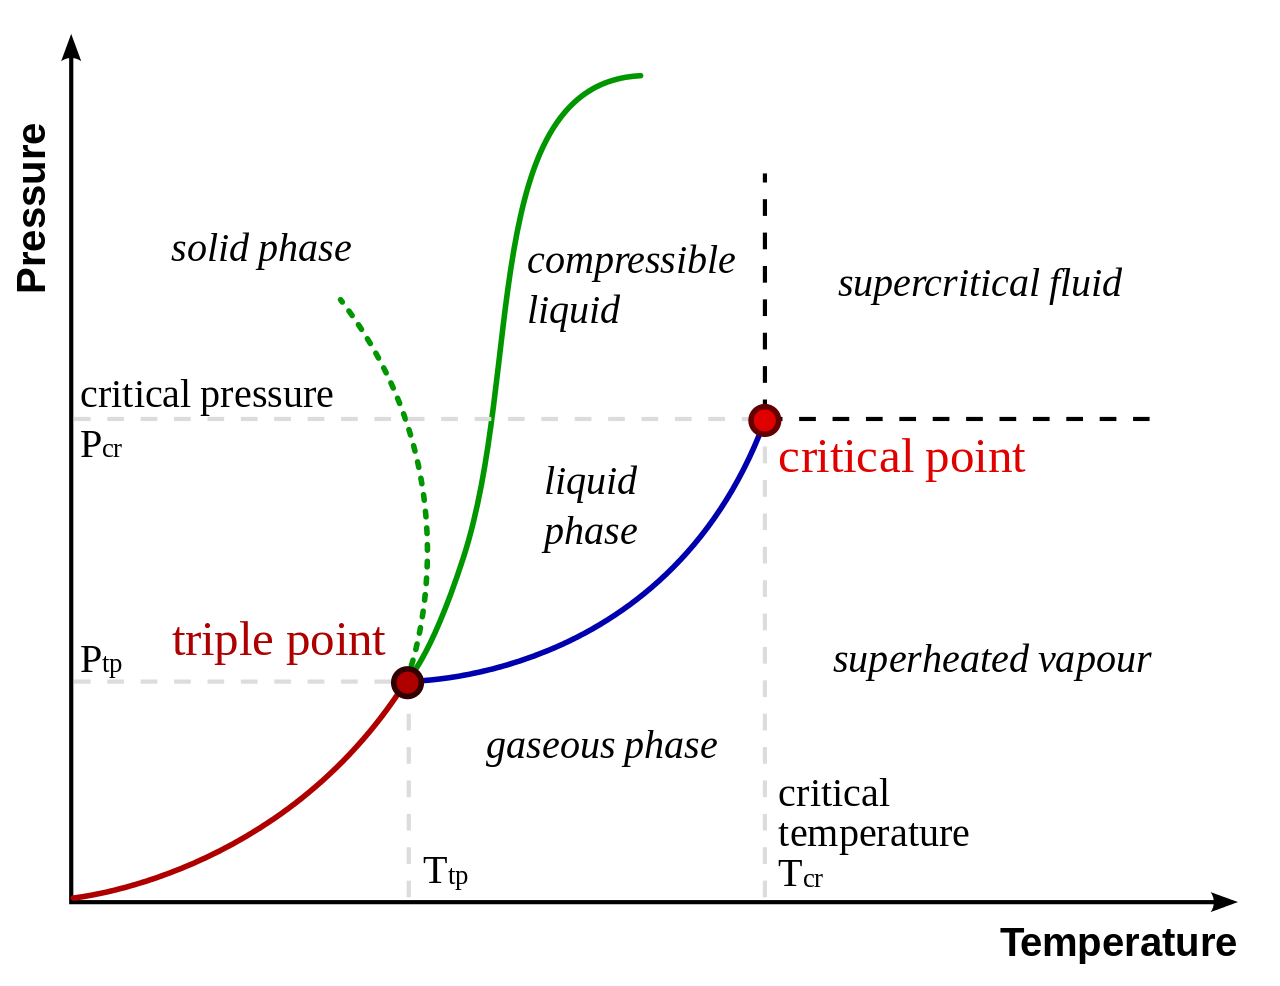
\includegraphics[width=0.5\textwidth]{diagfase.png}
\caption{\textit{Diagrama de Fases}}
\end{wrapfigure}
    \quad La temperatura a la cual cierto líquido hierve dependerá únicamente de la presión a la que esté sometido. A esta temperatura de saturación,  se llega cuando la sustancia en fase líquida entra en equilibrio dinámico con la fase gaseosa de la misma. \\ 
    \null \quad El diagrama de fases de la fig. 1 representa las diferentes fases de una sustancia en función de la temperatura y presión a la que está sometida. Se puede observar que la frontera entre la fase líquida y la fase gaseosa es una línea, lo que significa que a cada temperatura de saturación le corresponde una única presión de saturación. Otra cosa a observar es la línea verde punteada de pendiente negativa. Esta describe como la temperatura de fusión \emph{del agua} disminuye según aumenta la presión. 
    Dada una presión de vaporización(saturación), se podrá calcular la temperatura de saturación a través de la ecuación de \emph{Frost-Kalkwarf-Thodos}:
    \begin{equation}
        lnP^{vap} = A - \frac{B}{T} + ClnT + \frac{DP^{vap}}{T^{2}}
        \footnote{A, B, C, D, $A_{1}$, $A_{2}$, $A_{3}$ serán constante empíricas que varían con la sustancia\\
                \quad T es la temperatura, en K\\
                  \quad $P^{vap}$ es la presión de vaoprización, en mmHg}
    \end{equation}
    Por otro lado, se podrá obtener una primera aproximación de T usando la \emph{ecuación de Antoine:}
    \begin{equation}
        lnP^{vap}=A_{1} - \frac{A_2}{T+A_3} 
    \end{equation}
\pagebreak
\section{Métodos}
Antes de nada, me gustaría introducir los métodos que usaré a lo largo de esta práctica:
\begin{multicols}{2}
\subsection{Bisección}
%\begin{wrapfigure}{h}{0.5\textwidth}
%\centering
%\includegraphics[width=0.5\textwidth]{biseccion.PNG}
%\caption{\textit{biseccion.png}}
%\end{wrapfigure}
El método de la bisección consiste en iterar sobre dos puntos, $x_{1}$ y $x_{2}$. Se exige que entre ellos se encunetre la raíz(a través de que el valor de la función en un punto es diferente al valor de la función en el otro)(Teorema de Bolzano). La función \texttt{biseccion.m} calcula el punto medio de los dos puntos dados, busca cuál de los dos puntos tiene un signo diferente(del valor de la función), y se redefinirán los puntos. Este proceso continúa hasta que se cumpla $|x_{2}-x_{1}|<\epsilon$
\subsection{Secante}
El método de la secante, por otro lado, toma 2 puntos, $x_{1}$ y $x_{2}$. En vez de iterar sobre el punto medio, lo cual es bastante poco eficiente, traza una recta secante que pase por la imagen de los dos puntos dados, y halla la raíz de dicha recta. Tomará esta raíz como $x_{2}$, $x_{1}$ pasará a ser $x_{2}$, y vuelve a empezar. El proceso se repetirá hasta que se cumpla $|x_{2}-x_{1}|<\epsilon$
\end{multicols}
\pagebreak
\section{Procedimiento}
Queremos calcular la temperatura de saturación del etilbenceno($CH_{3}CH_{2}$) a una presión de 2494mmHg. Usaremos la aproximación (2) para encontrar un intervalo de amplitud 1 que contenga la raíz. Usaremos para esto un bucle while, y comenzaremos en un valor mayor a $A_{3}$, dado el carácter asintótico de la función. 


A Table of Contents and a bibliography have also been implemented. To add entries to your bibliography, simply edit \texttt{biblist.bib} in the root folder and then use the \texttt{\textbackslash cite\{\ldots\}} command in \texttt{main.tex} \cite{bibtex}. The Table of Contents will be updated automatically.

I hope that you find this template both visually appealing and useful. \\

\hspace{1 cm}--- Linus

\newpage
\bibliographystyle{plain}
\bibliography{biblist}

\end{document}